\chapter[Background information and literature review]{Background information and literature review}

\section{Introduction}
All liquid-fueled \gls{MSR} designs involve varying levels of online fuel processing. Minimally, volatile gaseous fission products (e.g. Kr, Xe) escape from the fuel salt during routine reactor operation and must be captured. Additional systems might be used to enhance removal of those elements. Most designs also call for the removal of rare earth metals from the core since these metals act as neutron poisons. Some designs suggest a more complex list of elements to process (figure~\ref{fig:periodic_tab}), including the temporary removal of protactinium from the salt or other regulation of the actinide inventory in the fuel salt \cite{ahmad_neutronics_2015}. This chapter contains a brief background 
information about \gls{MSR} online reprocessing system and a literature review.
\begin{figure}[htp!] % replace 't' with 'b' to 
  \centering
  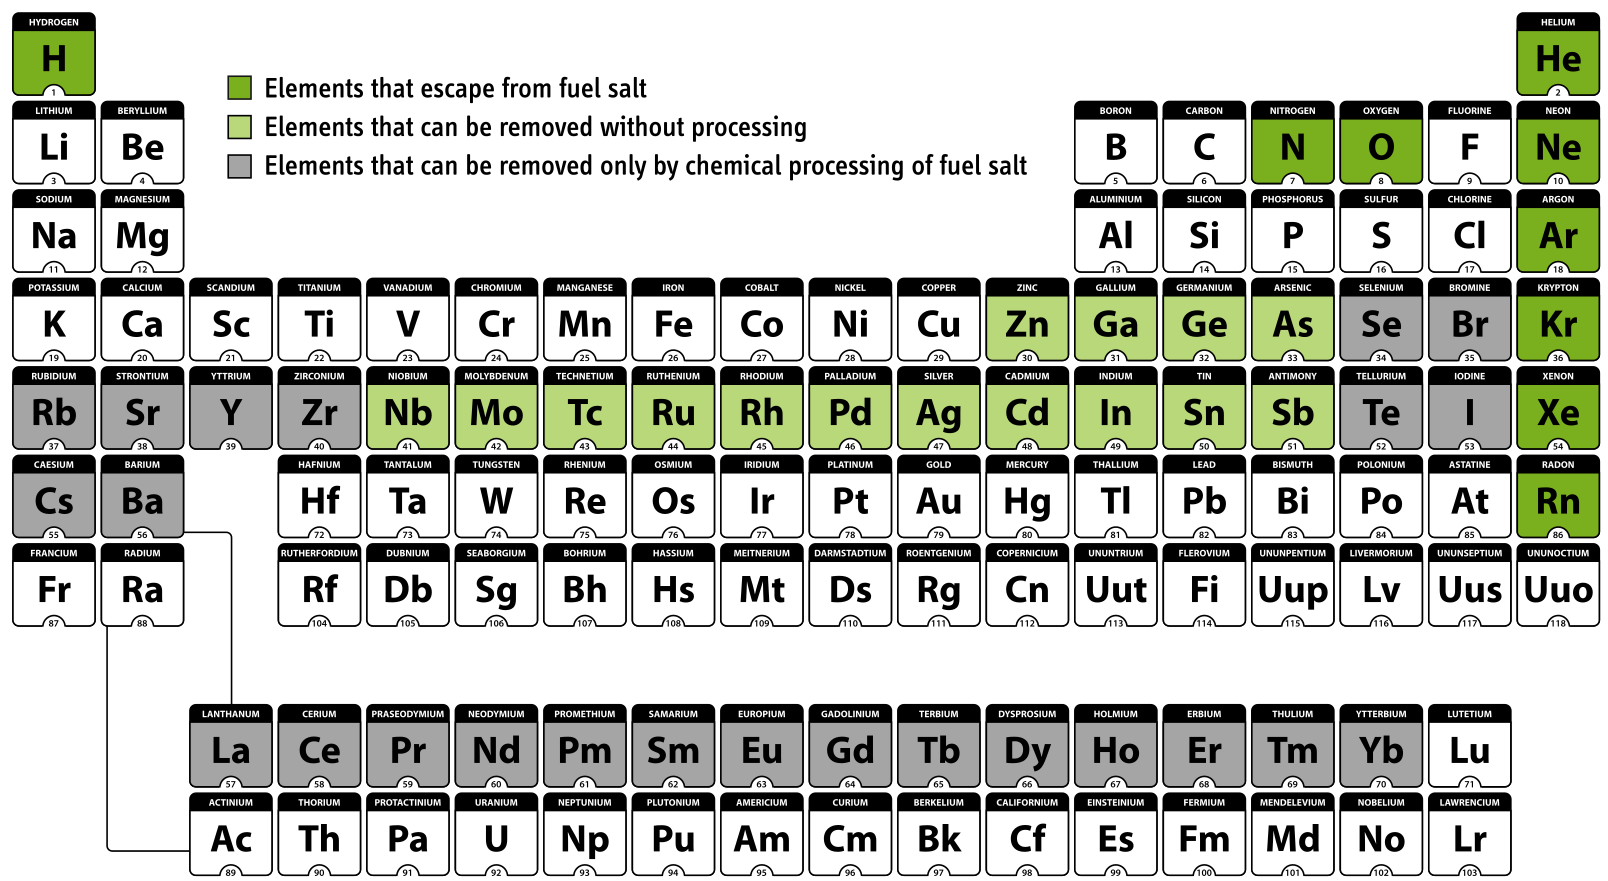
\includegraphics[width=0.87\textwidth]{periodic_map.png}
  \caption{Processing options for \gls{MSR} fuels (figure reproduced from 
  Ahmed \emph{et al.} \cite{ahmad_neutronics_2015}).}
  \label{fig:periodic_tab}
\end{figure}

\section{Online separations and feeds}
A liquid-fueled \gls{MSR} has online separations and/or feeds, where material 
is moved to or from the core at all times (continuous) or at specific intervals 
(batch). Contrarily, in a solid-fueled reactor, fission products and actinides 
remain within the initial fuel material during and after operation until 
reprocessing. The ability to perform online fuel salt reprocessing improves 
the potential neutronic performance of liquied-fueled reactors. Firstly, it 
is unnecessary for liquid-fueled reactors to operate with excess reactivity 
because fissile material is continuously being added into the core. Secondly, 
continuously removing fission products including strong absorbers (poisons) 
should significantly improve fuel utilization and decrease parasitic 
neutron absorption. Finally, neutronic parameters could be adjusted 
``on-the-fly" without operational cycle interruption. Nevertheless, removal 
of each element from the liquid fuel salt presents a unique challenge in 
terms of chemical separation processes, storage and disposal of the 
separated materials.

Modeling liquid-fueled systems with existing neutron transport and 
depletion tools is challenging because most of these tools are 
designed for the solid-fueled reactors simulation. The fuel material 
flows and potential online separations or feeds of specific elements 
or nuclides are the main challenges of liquid-fueled systems. 

\section{Literature review}
Most contemporary nuclear reactor physics software is 
unable to perform depletion calculations in an online 
reprocessing regime. Furthermore, existing tools for 
online refueling simulations are internally developed 
at universities and research institutions and not 
available for external use. The foundation for these in-house
tools was based on early \gls{MSR} simulation methods 
at \gls{ORNL}, which integrated neutronic and fuel 
cycle codes (i.e., Reactor Optimum Design (ROD) 
\cite{bauman_rod_1971}) into operational plant tools 
(i.e., Multiregion Processing Plant (MRPP) 
\cite{kee_mrpp_1976}) for \gls{MSR} and reprocessing 
system design. Based on this approach, recent tools 
from universities and research institutions can
approximate online refueling \cite{serp_molten_2014-1}. 
A summary of recent efforts is listed in table~\ref{tab:fs_codes}.
\begin{table}[ht!]
\caption{Tools and methods for liquid-fueled \glspl{MSR} fuel salt depletion analysis.}
\begin{tabularx}{\textwidth}{x s a a} 
\hline Neutronics software  & \qquad\qquad\qquad Authors & Spectrum & Removal   \\
        used for depletion  &                &          & efficiency  \\
\hline
\gls{MCNP}/REM \cite{noauthor_mcnp_2004,heuer_simulation_2010}  & Nuttin \emph{et al.}, 2005; Doligez 
\emph{et al.}, 2014; Heuer \emph{et al.}, 2014  
\cite{nuttin_potential_2005,doligez_coupled_2014,heuer_towards_2014}
& thermal/ fast & ideal \\
ERANOS \cite{ruggieri_eranos_2006}  & Fiorina \emph{et al.}, 2013 
\cite{fiorina_preliminary_2012-1}            
& fast & ideal \\
KENO-IV/ORIGEN \cite{goluoglu_monte_2011,gauld_isotopic_2011}     & Sheu 
\emph{et al.}, 2013 \cite{sheu_depletion_2013} 
& fast & ideal\\
SERPENT2 \cite{leppanen_serpent_2015}  & Aufiero \emph{et al.}, 2013
\cite{aufiero_extended_2013}; Ashraf \emph{et al.}, 2018 \cite{ashraf_nuclear_2018} & fast & ideal \\
DIF3D \cite{derstine_dif3d_1984} & Zhou \emph{et al.}, 2018 
\cite{zhou_fuel_2018-1} 
& thermal/ fast & ideal \\
MCODE/ORIGEN2 \cite{xu_mcode_2008,croff_users_1980} & Ahmad \emph{et al.}, 
2015 \cite{ahmad_neutronics_2015}   
& thermal & ideal \\
OpenMC/ORIGEN-S \cite{romano_openmc_2015,rearden_scale_2018}  & de Lanversin \emph{et al.}, 
2017 \cite{de_troullioud_de_lanversin_toward_2017}   
& thermal & ideal\\
\gls{MCNP}6/CINDER90 \cite{goorley_mcnp6_2013}     & Park \emph{et al.}, 2015; 
Jeong \emph{et al.}, 2016 \cite{park_whole_2015, jeong_equilibrium_2016}& 
thermal & ideal \\
SCALE/TRITON \cite{bowman_scale_2011,powers_new_2013}    & Powers \emph{et al.}, 
2014; Betzler \emph{et al.}, 2017; \qquad Li \emph{et al.}, 2018
\cite{powers_new_2013,powers_inventory_2014,betzler_molten_2017, li_optimization_2018} & thermal & ideal \\
SERPENT2     & Rykhlevskii \emph{et al.}, 2017-19 \cite{rykhlevskii_online_2017, rykhlevskii_full-core_2017, rykhlevskii_advanced_2018,rykhlevskii_modeling_2019} & 
thermal & ideal \\
\hline
\end{tabularx}
  \label{tab:fs_codes}
\end{table}
\FloatBarrier
\begin{sidewaystable}
	\centering
	\caption{\gls{MSR} online reprocessing simulation efforts published in 
	the literature.} 
	\vspace{1ex}
\begin{tabularx}{\textwidth}{a p{0.2\textwidth} x x x x x x x}
	\hline
	\textbf{Ref}  & \textbf{Neutronics software} & \textbf{Reactor} & \textbf{Geometry} & \textbf{Spectrum} &	\textbf{Reactivity} &\textbf{Reprocess-} &\textbf{Removal} \\
	 & \textbf{used for depletion} & \textbf{design} & & & \textbf{control} & \textbf{ing approach} & \textbf{efficiency} \\
	\hline
	\cite{nuttin_potential_2005}&\gls{MCNP}\cite{noauthor_mcnp_2004}&MSBR&unit-cell&thermal&o&continuous&ideal\\
	\hline	
\end{tabularx}
\label{tab:table2}
\end{sidewaystable}

References \cite{li_optimization_2018,de_troullioud_de_lanversin_toward_2017,doligez_coupled_2014,
heuer_towards_2014, sheu_depletion_2013, aufiero_extended_2013} provide some form of reactivity control, 
and methods \cite{doligez_coupled_2014,heuer_towards_2014,aufiero_extended_2013,ahmad_neutronics_2015, 
park_whole_2015,jeong_equilibrium_2016,rykhlevskii_modeling_2019,nuttin_potential_2005} use a set of all nuclides in depletion calculations. Batch-wise approach was used in 
references \cite{powers_new_2013,powers_inventory_2014,betzler_molten_2017, 
li_optimization_2018, park_whole_2015, jeong_equilibrium_2016,
rykhlevskii_advanced_2018, rykhlevskii_modeling_2019},
and references \cite{nuttin_potential_2005,doligez_coupled_2014,
heuer_towards_2014, fiorina_preliminary_2012-1, sheu_depletion_2013,
aufiero_extended_2013, zhou_fuel_2018-1, ahmad_neutronics_2015,
de_troullioud_de_lanversin_toward_2017} are employed a continuous online 
reprocessing approach. Finally, all published in the literature efforts 
are considered an ideal online fission product removal processing  (e.g., 
extraction efficiency is 100\%), hence, the proposed work goal is 
to close the gap.


\subsection{Batch-wise online reprocessing approach}
Many liquid-fueled \gls{MSR} designs rely on online fuel processing in which  
material moves to and from the core. That can be done continuously or at 
specific time steps (batch-wise). In a modeling of the batch-wise approach, 
the burn-up simulation stops at a given 
time and restarts with a new liquid fuel composition (after removal of discarded 
materials and addition of fissile/fertile materials). \gls{ORNL} researchers 
have developed ChemTriton, a Python-based script for SCALE/TRITON which uses the 
batch-wise approach to simulate a continuous reprocessing and refill for 
either single or multiple fluid designs. ChemTriton models salt 
treatment, separations, discharge, and refill using a unit-cell \gls{MSR} 
SCALE/TRITON depletion simulation over small time steps to simulate continuous 
reprocessing and deplete the fuel salt \cite{powers_new_2013}. Methods listed in 
references \cite{zhou_fuel_2018-1, sheu_depletion_2013,
park_whole_2015, jeong_equilibrium_2016, powers_inventory_2014,
betzler_molten_2017,rykhlevskii_modeling_2019} 
are also employed a batch-wise approach. This approach has a few disadvantages. 
First, this method assumes that material transfer from the reactor primary 
loop to the reprocessing plant is discrete and instantaneous. In reality, 
some small fraction of fuel salt is \textbf{continuously} flows to the 
reprocessing plant and approximately the same \textbf{continuous} material flow 
is returning back to keep mass balance in a primary loop. Second, this approach 
assumes that material accumulation in the core 
during the time between separations or feeds does not affect reactor physics which 
is not true for relatively long (few days) depletion simulation time steps. 
These assumptions for simulation of the nonstop online reprocessing process 
tends to misrepresent depleted material composition.

\subsection{Continuous online reprocessing approach}
Accounting for continuous removal or addition presents a greater challenge 
since it 
requires adding a term to the Bateman equations. In SCALE/TRITON, 
ORIGEN \cite{gauld_isotopic_2011} solves a set of Bateman equations using 
one-group averaged fluxes and cross-sections obtained from a transport 
calculation. The Bateman equations that describe the rate of change of the 
isotopes due to neutron induced reactions and decay processes can be 
written in the following form \cite{aufiero_extended_2013}:
\begin{align}
\frac{dN_i}{dt} &= \bar{\Phi}\sum\limits_{j}N_{j}\sigma_{j \rightarrow 		i} - \bar{\Phi}\sum\limits_{j}N_{i}\sigma_{i \rightarrow j} + \sum					\limits_{j}	N_{j}\lambda_{j}b_{j \rightarrow i} - N_{i}\lambda_{i} \\
& \qquad\qquad (1) \qquad\qquad\quad (2) \qquad\quad\qquad (3) \qquad\qquad (4) \nonumber
\label{eq:bateman}
	\intertext{where} 
	N_i &= \mbox{number density of isotope i} \\
	N_j &= \mbox{number density of isotope j} \\
	\bar{\Phi} &= \mbox {average in the space and energy neutron flux} \\
	\sigma_{j \rightarrow i} &= \mbox{microscopic one-group transmutation cross section} \\
	\lambda_i &= \mbox{decay constant of nuclide i} \\
	\lambda_j &= \mbox{decay constant of nuclide j} \\
	b_{j \to i} &= \mbox{branching fractions of radioactive decay from nuclide j}
\end{align}

The four terms on the right-hand side of the equation represent (1) the production rate of nuclide $i$ from irradiation, (2) the loss rate of nuclide $i$ due to irradiation, (3) the decay rate of nuclide $j$ into nuclide $i$, and (4) the loss rate of nuclide $i$ due to decay. Mentioned earlier, the deterministic codes  SCALE/TRITON and Monte Carlo codes MCNP, Shift, KENO-VI do not support 
removal or feed rates for depletion simulations.

Online fuel reprocessing can be explicitly introduced in the system of 
equations by adding effective decay and transmutation terms for the 
various nuclides. Fuel refill during fuel salt composition evolution 
calculations can be taken into account by
adding a gain term on the right-hand side of the Bateman equations:
\begin{align} 
\bar{\Phi}\sum\limits_{k=^{235}U}N_{k}\sigma_{k,c}  \label{eq:feed_term}
\end{align}
where $\sigma_{k,c}$ is the one-group capture cross section of feed 
isotope (e.g., $^{235}$U).

The removal of fission products is achieved by adding an explicit decay 
term to the Bateman equations. For the generic fission product, $l$, 
loss term can be added:
\begin{align} 
- N_{l}\lambda_{l,removal}  \label{eq:rem_term}
\end{align}
where $\lambda_{l,removal}$ is the effective removal time constant of the particular chemical species. 

Fiorina \emph{et al.} simulated \gls{MSFR} depletion with continuous fuel 
salt reprocessing via introducing 
``reprocessing'' time constants into the ERANOS transport code 
\cite{fiorina_preliminary_2012-1}. Nuttin \emph{et al.} used a similar approach 
to simulate online reprocessing with the MCNP Monte Carlo code for a 
\gls{MSBR}-like reference 
system with $^{232}$Th/$^{233}$U fuel \cite{nuttin_potential_2005}.
The same concept was adopted to model continuous feeds and extractions 
using the 
MCNP transport software listed in references \cite{doligez_coupled_2014,
heuer_towards_2014}. 

A similar method was recently implemented as a purpose-made extension within 
the continuous-energy Monte Carlo reactor physics and burn-up code 
SERPENT by explicitly introducing 
continuous reprocessing in the system of Bateman equations and adding 
effective decay and transmutation terms for each nuclide 
\cite{aufiero_extended_2013}. This was employed to study the material 
isotopic evolution of the \gls{MSFR}\cite{aufiero_extended_2013}. 
That SERPENT extension \cite{aufiero_extended_2013} directly 
accounts for the effects of online fuel reprocessing on depletion calculations 
and features a reactivity control 
algorithm. The extended version of SERPENT2 was assessed against a dedicated 
version of the deterministic ERANOS-based EQL3D procedure in
\cite{ruggieri_eranos_2006, fiorina_investigation_2013} and adopted to analyze 
the \gls{MSFR} fuel salt isotopic evolution. In addition, the latest SCALE release 
will also have the same functionality using truly continuous removals \cite{betzler_implementation_2017}. 

Nuttin \emph{et al.} broke up the reactor core geometry into three \gls{MCNP} cells: 
one for salt channels, one for the salt plena above and below the core, and a 
third cell for the annulus. Consequently, the two-region reactor core was 
approximated by one region with averaged fuel/moderator ratio 
\cite{nuttin_potential_2005}. Similarly, Powers \emph{et 
al.}, Betzler \emph{et al.}, and Jeong \emph{et al.} 
\cite{powers_new_2013,powers_inventory_2014,betzler_modeling_2016, 
betzler_molten_2017, jeong_development_2014, jeong_equilibrium_2016} used a 
simplified unit-cell models. This approach 
misrepresents the two-region breeder reactor concept. The unit-cell or one-region 
models may produce reliable results for homogeneous reactor cores (i.e. 
\gls{MSFR}, \gls{MOSART}) or for one-region single-fluid reactor designs (i.e. 
\gls{MSRE}). However, many reactor concepts with sophisticated geometry (e.g., 
two-region \gls{MSBR}, \gls{TAP} \gls{MSR} with irregular moderator pattern) must 
be simulated using a whole-core model to accurately capture different neutron 
transport characteristics in the different regions of the core. Therefore, in 
general, the online reprocessing tools and reactor physics codes should be tested 
using high-precision full-core reactor core models.

\subsection{Extraction efficiency}
Chemical extraction of neutron poison from the fuel salt can be 
done with extraction efficiency ($\epsilon$) which is defined as 
follows:
\begin{align}
\epsilon &= \frac{n_{ext}(M)}{n_{init}(M)}
\label{eq:efficiency}
\intertext{where} 
	n_{ext} &= \mbox{the number of moles of the element M extracted}  \nonumber \\
	n_{init}&= \mbox{the initial number of moles of the element M} \nonumber
\end{align} 
All references listed in Table~\ref{tab:fs_codes} are assumed an extraction efficiency
 equal 100\% (e.g. 100\% of mass of target isotopes 
removed within the ``cycle times''\footnote{ The \gls{MSBR} 
program defined a ``cycle time" as the amount of 
time required to reprocess entire salt ($T_r$) 
\cite{robertson_conceptual_1971}.}). 
Nuttin \emph{et al.} introduced separation efficiency ($\epsilon_e$) using the 
equation below \cite{nuttin_potential_2005}:
\begin{align}
dN_e = N_{e, 0} \frac{dt}{T_r} \epsilon_e
\end{align}
where $dN_e$ is the extracted amount of element $e$; 
$N_{e, 0}$ is the initial inventory of the element $e$; 
$dt$ is the time interval; 
$T_r$ is the time needed to reprocess entire salt (cycle time). 
Integration of both parts of this equation leads to the
following expression for the amount of element $e$ after extraction:
\begin{align}
N_{e, 1} = N_{e, 0} e^{\frac{\epsilon_e}{T_r}t}
\end{align}
For the simplified case when the efficiency selected equals 
100\%, the effective removal time constant 
($\lambda_e$) for the element $e$ can be estimated as follows:
\begin{align} 
\lambda_e = \epsilon_e / T_r  \label{eq:100_lam}
\end{align}
For the case with realistic separation efficiency (e.g., 99\% for 
uranium extraction), the effective removal time constant for the 
element $e$ can be expressed as \cite{nuttin_potential_2005}:
\begin{align}  
\lambda_e = \frac{ln |1-\epsilon_e|}{T_r} \label{eq:real_lam}
\end{align}
Equation \ref{eq:real_lam} is an exponential extrapolation and has been 
used to estimate removal constant for the
extraction term in the Bateman equations (\ref{eq:rem_term}) in references \cite{nuttin_potential_2005, betzler_implementation_2017, doligez_coupled_2014}.

\subsection{Online reprocessing tool simulation flow charts}
Liquid-fueled systems present a challenge to existing neutron transport 
and depletion tools, which are typically designed to simulate 
solid-fueled reactors. To handle the material flows, and the online 
removal/feed of an \gls{MSR}, researchers developed in-house 
tools which usually built on top of existing neutron transport and 
depletion software. Figure~\ref{fig:typical_flow_chart} demonstrates typical 
flow charts for batch-wise (references \cite{betzler_molten_2017,
li_optimization_2018,rykhlevskii_modeling_2019,zhou_fuel_2018-1,
sheu_depletion_2013,park_whole_2015}) and 
online reprocessing (references \cite{heuer_simulation_2010,
doligez_coupled_2014,  heuer_towards_2014, fiorina_investigation_2013,
nuttin_potential_2005, aufiero_extended_2013,
de_troullioud_de_lanversin_toward_2017}) tools. Almost all existing 
software tools represent chemical reprocessing plant as ``black box'' 
model (orange ellipses on figure~\ref{fig:typical_flow_chart}) which 
removes target 
elements all at once with constant efficiency. Typical inputs and outputs 
for this ``black box'' model are vectors of elements and extraction 
efficiencies and can be 
expressed as follows:
\begin{equation}
\begin{bmatrix}
N^{in}_{element \: 1} \\ N^{in}_{element \: i} \\ \vdots \\
\end{bmatrix} 
\times
\begin{bmatrix}
\epsilon_{element \: 1} \\ \epsilon_{element \: i} \\ \vdots \\
\end{bmatrix} =
\begin{bmatrix}
N^{out}_{element \: 1} \\ N^{out}_{element \: i} \\ \vdots \\
\end{bmatrix}
\end{equation}
where $N^{in/out}_i$ is the number of atoms of $i^{th}$ element and 
$\epsilon_i$ is the 
extraction efficiency for $i^{th}$ element. There are few issues with 
simplified ``black box'' model: 
\begin{enumerate}
	\item Previous work in the literature assumed that separation 
efficiency vector is not changing with time and does not depend on reactor 
operational parameters (separation efficiency might changes with temperature, 
power level, current fuel salt isotope composition, etc).

	\item Fuel salt in a reprocessing plant undergoes not a single but many 
	separate processes (e.g. He bubbling, nickel mesh filter, etc). Some of 
	these processes can be done in parallel but many in series.
	
	\item Ignoring the decay of radioactive nuclides during processing in  
	the reprocessing plant (chemical separation is not an instantaneous process) 
	especially processing in series. 
	
	\item Each chemical process is related with a chemical processing volume 
	which has limited volume (for batch process) and/or capacity (for 
	continuous process). 
	Moreover, separation efficiency of the facility depends on material flow 
	rate (higher mass flow rate leads to lower separation efficiency 
	\cite{briggs_molten-salt_1969}).
\end{enumerate}

\begin{figure}[hbp!] % replace 't' with 'b' to \centering
  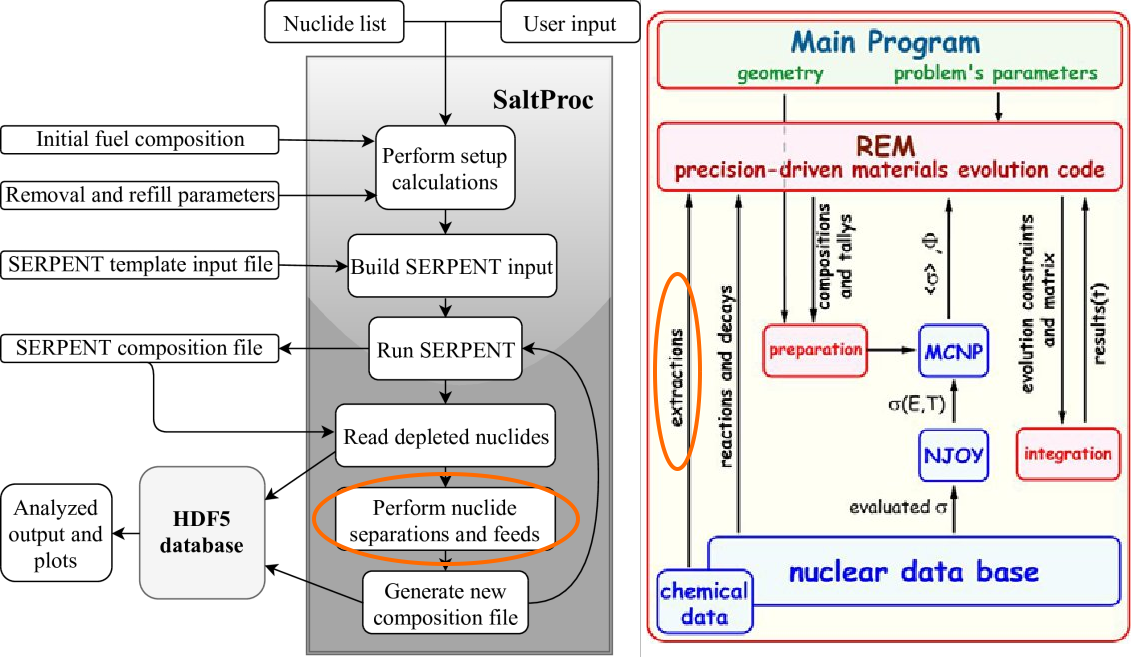
\includegraphics[width=\textwidth]{typical_flow_chart.png}
  \caption{Typical flow charts of online reprocessing simulation tool:
  batch-wise tool SaltProc (uses SERPENT2 for neutron transport and 
  depeletion) \cite{rykhlevskii_modeling_2019}
   (left) and continuous  REM (uses MCNP as transport code) 
   \cite{heuer_simulation_2010} (right).} 
  \label{fig:typical_flow_chart}
\end{figure}

For the realistic simulation, ``black box'' with only separation efficiency 
as a parameter should be substituted with different boxes each representing 
particular unit of
separation equipment. Simon \emph{et al.} made an effort to develop a 
reprocessing software package for realistic \gls{MSBR} reprocessing 
plant simulation which based on chemistry models \cite{simon_-line_2008}. 
The code represents two simple separation processes: (1) protactinium 
extraction by reductive salt-metal extraction in a bismuth medium (original 
\gls{MSBR} method proposed by \gls{ORNL} \cite{whatley_engineering_1970-1}), 
and (2) lanthanide extraction based on a 2-step recovery process: 
the reduction of 
lanthanides by lithium from the fluoride fuel salt to liquid bismuth, then the 
oxidation of lanthanides from liquid bismuth to a lithium chloride salt. Simon and 
colleagues applied this code to an \gls{MSBR}-like reactor design and 
obtained realistic 
correlations for protactinium and lanthanide extraction efficiencies. Those 
correlations are required data describing for mass flow rates for the salt 
and liquid metal (Bi), the distribution coefficient between fluoride salt 
and Bi-Li-Th, the interfacial areas 
between fluoride salt and Bi-Li-Th, and the mass transfer coefficient through the 
interface. Unfortunately, this research effort only modeled reprocessing plant 
and was not coupled with a neutronics code to simulate fuel salt depletion in 
the reactor core. An online reprocessing tool, which simulates fuel salt 
depletion in the core and realistically models a reprocessing plant, 
would allow modeling of the comprehensive behavior of  
Molten Salt liquid-fueled systems.
